\documentclass[11pt]{article}

\usepackage{times}
\usepackage{graphicx}

\textwidth=6.5in
\textheight=8.75in
\oddsidemargin=0.0in
\evensidemargin=0.0in
\topmargin=-0.5in

\begin{document}
\thispagestyle{empty}

\begin{center}
{\bf CS 6300} \hfill {\large\bf HW02:  CSPs and Minimax} \hfill {\bf Due February 1, 2022}
\end{center}

Please use \LaTeX\ to produce your writeups. See the Homework Assignments 
page on the class website for details.

\section{CSPs}

You are in charge of scheduling arrivals for Pohonk Internation
Airport.  The airport has two runways (R and L), and four landing time
slots (T1, T2, T3, T4).  Today, there will be 4 arrivals, each of
which you must assign a runway and a time slot.  Here are the
requirements for the schedule:

{\small

\begin{center}\begin{tabular}{ll}
1. & Air Force One (AF1) must land on runway R due to motorcade and secret service logistics. \\
2. & The airport closes (no landings) for one timeslot before, one during, and one after the arrival of AF1. \\
3. & The Blue Angels (BA) will land in formation, which requires both runways at the same time. \\
4. & The Blue Angels are exempt from AF1 related airport closures. \\
5. & The new Boeing 777 Dreamliner (B777) must land before the Blue Angels. \\
6. & The B777 must land on runway L. \\
7. & The Cessna (C) must not land beside or one timestep after the B777, due to turbulence considerations. \\
8. & No two planes may land on the same runway at the same time. 
\end{tabular}\end{center}

}

\begin{center}
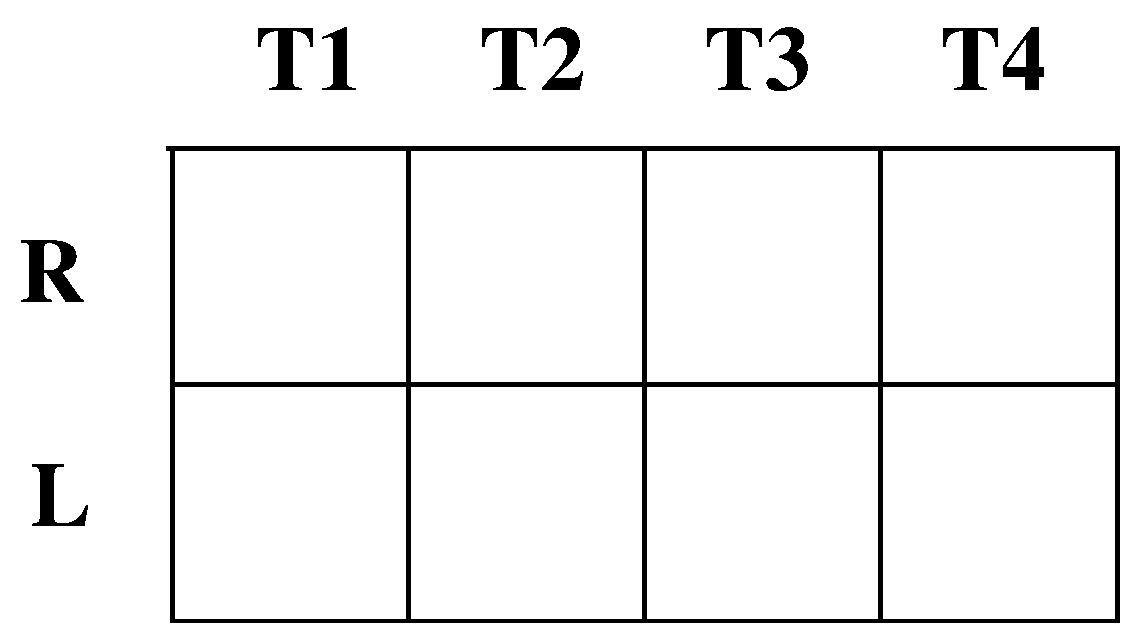
\includegraphics[width=3in]{Airport.eps}
\end{center}

\begin{enumerate}

\item Represent the problem with 4 variables: AF1, B777, C, and
  BA. The domain of BA is a time between 1 and 4 that the Blue Angels
  will arrive; the domain of the other three variables is a time
  between 1 and 4 plus `R' or `L' to specify the runway being landed
  on.  Enumerate separately the unary and binary constraints in this
  problem. For the binary constraints, you may use pseudocode for
  implicit functions, like {\it beside(?,?)}.

  \paragraph{Unary Constraints:}

  \begin{flushleft}\begin{tabular}{ll}
  ?  & ? \\
  ?  & ? \\
  ?  & ? \\
  \end{tabular}\end{flushleft}

  \paragraph{Binary Constraints:}

  \begin{flushleft}\begin{tabular}{ll}
  ?  & ? \\
  ?  & ? \\
  ?  & ? \\
  \end{tabular}\end{flushleft}

\item Write constraint 5 in explicit form. \\

\item Enforce all {\it unary} constraints by deleting values in the table below.

\begin{center}\begin{tabular}{l|cccccccc|}
{\bf AF1}  & R1 & R2 & R3 & R4 & L1 & L2 & L3 & L4 \\ 
{\bf B777} & R1 & R2 & R3 & R4 & L1 & L2 & L3 & L4 \\ 
{\bf C}    & R1 & R2 & R3 & R4 & L1 & L2 & L3 & L4 \\ 
{\bf BA}   & R1\&L1 & R2\&L2 & R3\&L3 & R4\&L4 &  &  &  &  \\ 
\end{tabular}\end{center}

\item Transfer your answer from part 3 to the table below. Then run
  arc-consistency.  Show your sequence of steps; i.e., the arc you
  picked and the resulting domain change.

  \begin{enumerate}

  \item Arc $X->Y$:  X loses value ?? due to constraint ??.

  \item Etc.
 
  \end{enumerate}

\begin{center}\begin{tabular}{l|cccccccc|}
{\bf AF1}  & R1 & R2 & R3 & R4 & L1 & L2 & L3 & L4 \\ 
{\bf B777} & R1 & R2 & R3 & R4 & L1 & L2 & L3 & L4 \\ 
{\bf C}    & R1 & R2 & R3 & R4 & L1 & L2 & L3 & L4 \\ 
{\bf BA}   & R1\&L1 & R2\&L2 & R3\&L3 & R4\&L4 &  &  &  &  \\ 
\end{tabular}\end{center}

\item Assuming you have not yet found a unique solution, perform
  backtracking search, and maintain arc-consistency after each
  variable assignment. Use the Minimum Remaining Values (MRV)
  heuristic to choose which variable to assign first, breaking ties in
  the order AF1, B777, C, BA.  After each variable assignment,
  reassign the domains in the grid.

  \begin{enumerate}

  \item Variable assignment:  ??

\begin{center}\begin{tabular}{l|cccccccc|}
{\bf AF1}  & R1 & R2 & R3 & R4 & L1 & L2 & L3 & L4 \\ 
{\bf B777} & R1 & R2 & R3 & R4 & L1 & L2 & L3 & L4 \\ 
{\bf C}    & R1 & R2 & R3 & R4 & L1 & L2 & L3 & L4 \\ 
{\bf BA}   & R1\&L1 & R2\&L2 & R3\&L3 & R4\&L4 &  &  &  &  \\ 
\end{tabular}\end{center}

   \item Next variable assignment, etc.

   \end{enumerate}

\end{enumerate}

\clearpage

\section{Minimax}

Consider the two-player minimax game tree below.  Suppose the top node
is labeled $A$, the nodes at the next level $A_1, A_2, A_3$ from left
to right, the nodes at the next level under $A_1$ as $A_{11}, A_{12},
A_{13}$ from left to right, the nodes under $A_2$ as $A_{21}, A_{22},
A_{23}$, etc.  The terminal nodes have 3 indexes $A_{ijk}$.

\centerline{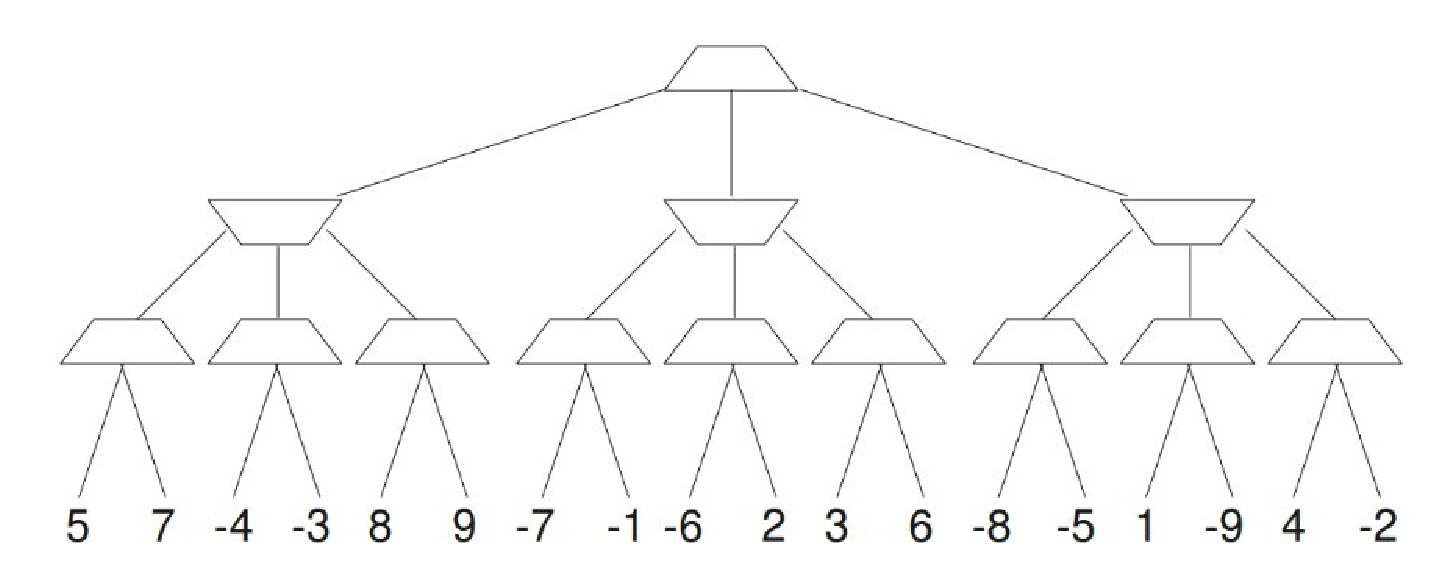
\includegraphics[width=0.9\textwidth]{minimax.eps}}

\begin{enumerate}

\item Carry out minimax search.  Give the values for each node.

\item Now use $\alpha-\beta$ pruning.  Let $ab_{i}$ be the
  $\alpha-\beta$ values passed down an edge to node $i$, etc., for all
  the nodes with appropriate change of index or indices.  Similarly,
  $v_i$ is the value passed up edge $i$, etc..  Show the sequence of
  steps, by giving the $ab$ values on the way down, and the $v$ values
  on the way up.

\end{enumerate}

\end{document}
